All posisjonering handler om å finne posisjonen til et objekt i forhold til et annet objekt. 
Den vanligste teknologien for lokalisering på jorden er GNSS (Global Navigation Satelite System), 
ofte bare omtalt som GPS (Global Positioning System). Ved bruk av GNSS kan man finne en posisjon i forhold til jorden, 
altså hvor på jorden man befinner seg. Når UWB brukes til posisjonering opprettes det et LPS (lokalt posisjonerings system). 
Man finner da posisjonen i forhold til dette posisjoneringssystemet, som er nyttig dersom man ønsker å finne posisjonen innendørs der det ikke er GNSS, 
eller ved tilfeller hvor det er viktigere å vite posisjonen i forhold til en konstruksjon enn jorden. Et UWB LPS er satt opp ved bruk av ankere som 
illustrert i figur \ref{fig:ankere}. Et anker velges som origo, og posisjonen til de andre ankerene måles opp i forhold til origo. 
En tag som beveger seg rundt i dette rommet vil kunne bruke ankerene til å regne ut sin egen posisjon. 
Måten dette gjøres på er at tagen først bruker TWR til å finne avstanden til hvert anker. Både disse avstandene og de kjente posisjonene til 
ankrene blir deretter brukt til å regne ut tagens posisjon i forhold til origo.

\begin{figure}[h]
\centering
\subfloat[Ved bruk av et anker kan tagen finne ut hvor langt unna ankeret den er.]{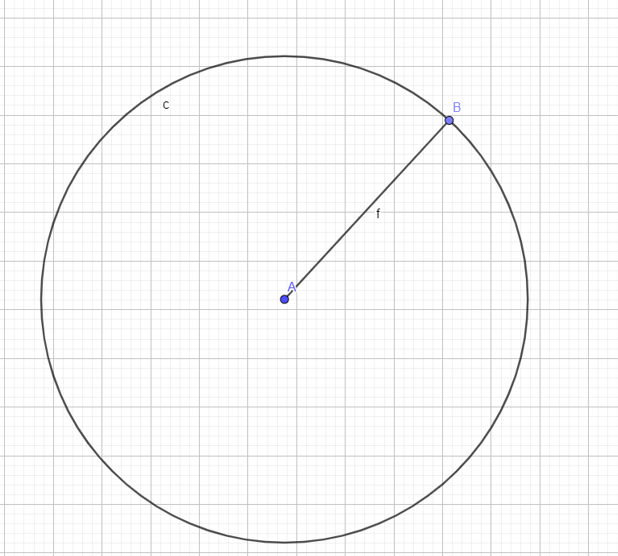
\includegraphics[width=.45\columnwidth]{1anker}} \quad
\subfloat[Ved bruk av to ankere med kjent posisjon kan tagen regne ut to mulige posisjoner den kan være på i 2D.]{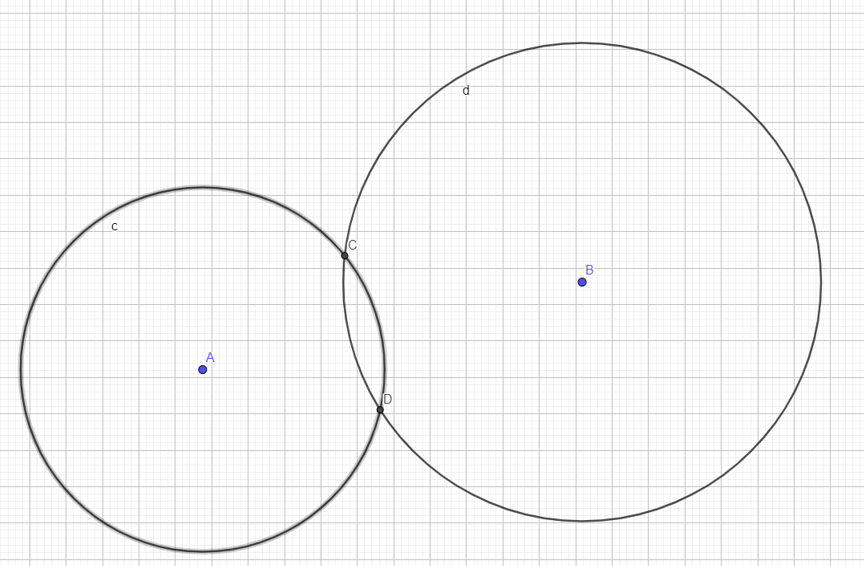
\includegraphics[width=.45\columnwidth]{2anker}\label{fig:ipsum}} \\
\subfloat[Ved bruk av tre ankere med kjent posisjon kan tagen regne ut en absolutt posisjon i 2D.]{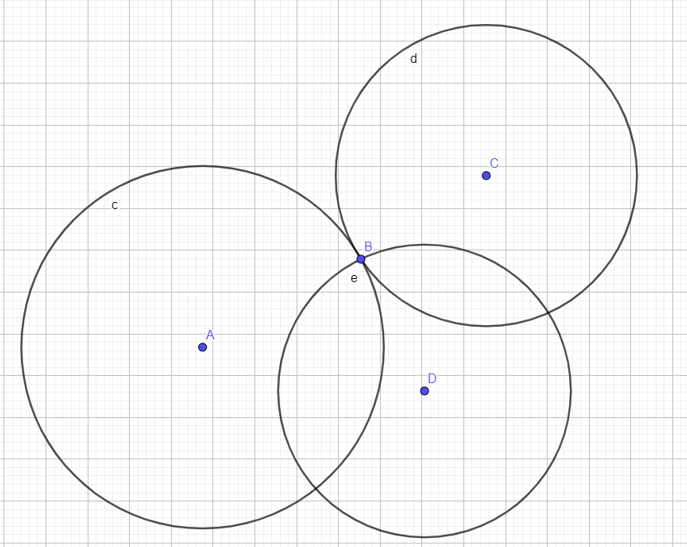
\includegraphics[width=.45\columnwidth]{3anker}} \quad
\subfloat[Ved bruk av 4 eller flere ankere med kjent posisjon kan tagen regne ut en posisjon i 3D, altså i x-retning, y-retning og høyde.]{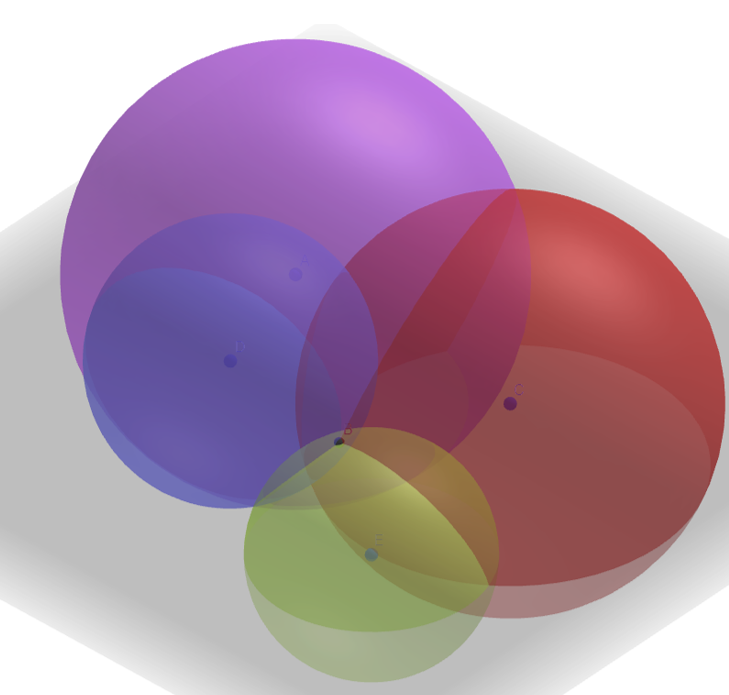
\includegraphics[width=.45\columnwidth]{4anker}}
\caption[Posisjonering ved ulike antall ankere.]{Posisjonering ved ulike antall ankere.} % The text in the square bracket is the caption for the list of figures while the text in the curly brackets is the figure caption
\label{fig:ankere}
\end{figure}